\documentclass{article}
\usepackage[margin=.75in]{geometry}
\usepackage{graphicx, dblfloatfix}
\usepackage{amsmath, amssymb, amsfonts, mathrsfs, mathtools}
\usepackage[english]{babel}
\usepackage[autostyle, english = american]{csquotes}
\usepackage[normalem]{ulem}
\usepackage[title,titletoc,toc]{appendix}
\usepackage{pgfplotstable}
\usepackage{array, booktabs, colortbl}
\MakeOuterQuote{"}

\pgfplotsset{compat=1.12}


\newcommand{\redchi}{$\tilde{\chi}^2\,$}
\DeclareMathOperator{\erf}{erf}
\DeclareMathOperator{\cov}{cov}
\DeclarePairedDelimiter\abs{\lvert}{\rvert}%
\DeclarePairedDelimiter{\parens}{\lparen}{\rparen}

\title{Single Photon Interference}
\author{Aman LaChapelle}

\begin{document}
\raggedright
\maketitle

\begin{abstract}
	We present here a method by which we can determine the wave-particle duality of light and show that it is a quantum-mechanical and that they comprise parts of a system that is not possible to describe classically.  In all, we are able to show several effects, each can be described classically on its own, but the combination of all these effects can only be described using quantum mechanics.
\end{abstract}

\tableofcontents
\newpage

\section{Introduction}
	It is generally well known that light has both particle-like qualities, in that it carries momentum, and that it can act like a quantum mechanical particle system in that its motion and other properties can be described in real space as well as in momentum space (roughly) with the free particle hamiltonian, especially in the regime where we have not engineered photon-photon interactions.  In general, we can use a faily standard probablistic interpretation in order to understand the way that light behaves given different situations.  In our particular case, we can understand the physical differences between distinguishable paths, indistinguishable paths, and ***erasure of interference that we can directly cause with a polarizing filter.


\section{Theory}
	An important property of interfering a photon with itself is that if we perform the experiment in such a way that the paths of the photon \emph{could} be distinguished, we do not in fact actually have to realize measurement of the difference between the paths of the photon.  In essence, what we can and will do is impose a polarization condition on the two arms of the interferometer.

	\subsection{Classical Photons}
	What we have discussed so far is, however, a quantum mechanical observation.  We can describe each of these situations classically by considering the polarization and co-propagation of the EM waves that make up the laser beam.  We will consider each of the three cases separately and begin to explore the classical electrodynamic explanation for these three phenomena.

	\hspace{.5cm}

	The first case we will consider is the case where the two paths the photon could take are indistinguishable.  Take the polarization of the photon(s) to be uniform across the two paths, and take the $\hat{z}$ to be the direction of propagation of the waves, so our wave vector $\vec{k} = \abs{k}\hat{z}$.  If we make the reasonable assumption that these photons propagate in what is approximately free space, we can write down the $\vec{E}$ and $\vec{B}$ fields like so:

	\begin{gather*}
		\vec{E} \, \text{or} \, \vec{B} = Ae^{i(\vec{k} \cdot \vec{r} - \omega t)} + Be^{-i(\vec{k} \cdot \vec{r} - \omega t)}\\
		\vec{E} = \parens*{Ae^{i(kz-\omega t)} + Be^{-i(kz-\omega t)}}\hat{x}\\
		\vec{B} = \parens*{Ae^{i(kz-\omega t)} + Be^{-i(kz-\omega t)}}\hat{y}
	\end{gather*}

	where we have arbitrarily chosen that the photon is polarized in $\hat{x}$.  Because we can simply choose our axes such that this occurs, we would be able to arbitrarily realign such that this is the case, or any of the orthogonal directions points along the polarization direction.  The most important thing to note here is that the $\vec{E}$, $\vec{B}$, and $\vec{k}$ are all orthogonal.  $A$ and $B$ are arbirtary scale constants.  There are relations between the $\vec{E}$ and $\vec{B}$ fields that we simply absorb into these constants.




\section{Apparatus}

\begin{figure}[!htb]
	\centering
	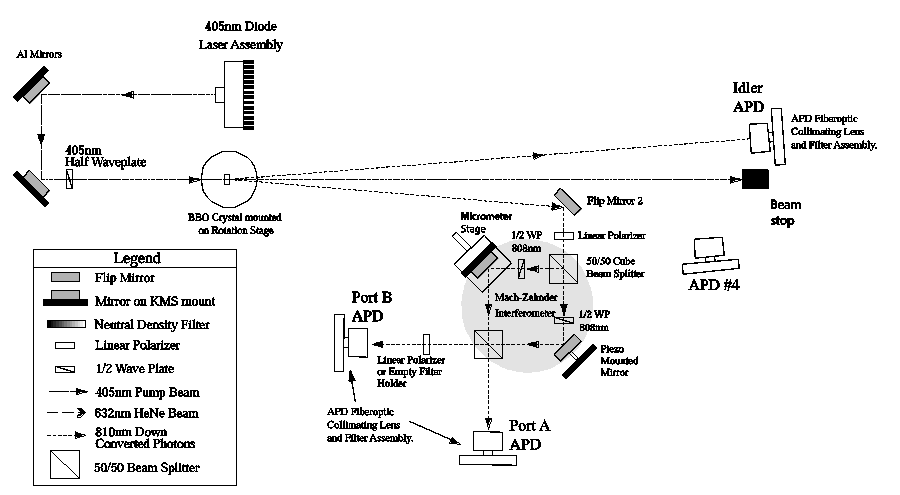
\includegraphics[scale=.5]{apparatus_setup.png}
	\caption{A schematic of the optical table as seen from above.  The APD letters correspond to numbers.  We attempt to keep the naming convention that uses the numerical representation, however.}
\end{figure}

\section{Data/Uncertainty Analysis}

\begin{table}
	\centering
	\pgfplotstabletypeset[
   		precision=2,
   		every head row/.style={before row=\toprule, after row=\midrule},
   		every row no 4/.style={after row=\midrule},
   		every last row/.style={after row=\bottomrule},
   		columns/0/.style ={column type = {|c|},column name=Parameters},
   		columns/1/.style ={column type = {|c|}, column name=Covariance Matrix},
   		columns/2/.style ={column type = {|c|}, column name=},
   		columns/3/.style ={column type = {|c|}, column name=},
   		columns/4/.style ={column type = {|c|}, column name=},
   		columns/5/.style ={column type = {|c|}, column name=},
   		every even row/.style={before row={\rowcolor[gray]{0.9}}}]{../data/fitparms.csv}
   		\caption{Zeroes indicate non-members of the covariance matrices.}
\end{table}

\section{Conclusion}

\begin{thebibliography}{10}
	\bibitem{first}
		stuff goes here

\end{thebibliography}

\end{document}